
	El algoritmo de Kalman se basa en poder estimar el vector de estados a partir de la dinámica del sistema y las mediciones. Para la definición del algoritmo utilizaremos la siguiente notación. Llamaremos:
	
	\begin{equation*}
		\vect{x_{k/k - 1}}
	\end{equation*}
	
	A la mejor estimación de el vector de estados utilizando información hasta el instante $k - 1$. Es decir se trata de una predicción. Llamaremos a la matriz de covarianza del error de dicha estimacion:
	
	\begin{equation*}
		\vect{P_{k/k - 1}}
	\end{equation*}
	
	Por otro lado llamaremos a:
	
	\begin{equation*}
		\vect{x_{k/k}}
	\end{equation*}
	
	A la mejor estimación del vector de estados utilizando información hasta el instante $k$. Dicha estimación será el resultado final del algoritmo y la matriz de covarianza del error del mismo será:
	
	\begin{equation*}
		\vect{P_{k/k - 1}}
	\end{equation*}

	Cabe aclarar que cuando decimos mejor estimador, hacemos referencia a que se trata del que minimiza el error cuadrático medio. Dicho todo esto, presentamos el algoritmo de Kalman para poder realizar la estimación de la trayectoria.
	
		\subsection{Algoritmo de Kalman}
			\paragraph{Inicialización}
				Es la etapa en la que definimos el estado inicial de la estimación, para poder inicializar el algoritmo necesitamos una estadistica del estado inicial del sistema:
				
				\begin{equation*}
					\vect{x_{0/0}} \leftarrow E\left[\vect{x_{0}}\right]
				\end{equation*}
				
				\begin{equation*}
					P_{0/0} \leftarrow COV\left[\vect{x_{0}}\right]
				\end{equation*}
			\paragraph{Predicción}
				Es la etapa en la que realizarmos una predicción del futuro estado del sistema utilizando el modelo en el espacio de estados:
				
				\begin{equation*}
					\vect{x_{k/k - 1}} \leftarrow Ad_{k - 1} \vect{x_{k - 1/k - 1}}
				\end{equation*}
				
				\begin{equation*}
					P_{k/k - 1} \leftarrow Ad_{k - 1} P_{k - 1 / k - 1} Ad_{k - 1}^{*} + Bd_{k - 1} Q_{k - 1} Bd_{k - 1}^{*}
				\end{equation*}
			\paragraph{Corrección}
				Es la etapa en la que corregimos la predicción con el valor de la medición, para ello necesitamos calcular la matriz de ganancia de Kalman $K_{k}$:
				
				\begin{equation*}
					K_{k} \leftarrow P_{k / k - 1} Cd_{k}^{*} (Cd_{k} P_{k/k - 1} Cd_{k}^{*} + R_{k})^{-1}
				\end{equation*}
				
				Luego corregimos:
				
				\begin{equation*}
					\vect{x_{k/k}} \leftarrow \vect{x_{k/k - 1}} + K_{k} (y_{k} - Cd_{k} \vect{x_{k/k - 1}})
				\end{equation*}
				
				\begin{equation*}
					P_{k/k} \leftarrow (I - K_{k} Cd_{k}) P_{k/k - 1}
				\end{equation*}
					
			\paragraph{Actualización}
				Es la etapa del algoritmo que pasamos al siguiente instante k.
				
				\begin{equation*}
					\vect{x_{k - 1/k - 1}} \leftarrow \vect{x_{k/k}}
				\end{equation*}
				
				\begin{equation*}
					P_{k - 1/k - 1} \leftarrow P_{k/k}
				\end{equation*}
	
	A continuación presentamos el script de MATLAB que implementa el algoritmo. Se puede seleccionar si se esta midiendo posicion, velocidad o aceleracion.

	\begin{lstlisting}[caption=\emph{Script} para la resolución del ejercicio 2]
%%%%%%%%%%%%%%%%%%%%%%%%%%%%%%%%%%
% EJERCICIO 2
%%%%%%%%%%%%%%%%%%%%%%%%%%%%%%%%%%
bool_p = 1;	% Inciso a
bool_v = 0;	% Inciso b
bool_a = 0;	% Inciso c


x0 = [40 -200 0 0 0 0]';
P0_0 = diag([100^2 100^2, 1 1, 0.1 0.1]);

%%%%% y_k = [I 0 0] [pk vk ak]' + ruido \eta
sigma_etap = 60;
sigma_etav = 2;
sigma_etaa = 0.1;

Bk1 = eye(cant_estados);
C =	[eye(dim*bool_p) zeros(dim*bool_p) zeros(dim*bool_p);
	 zeros(dim*bool_v) eye(dim*bool_v) zeros(dim*bool_v);
	 zeros(dim*bool_a) zeros(dim*bool_a) eye(dim*bool_a)];

M_eta = [randn(dim,cant_mediciones)*sigma_etap*bool_p; 
	randn(dim,cant_mediciones)*sigma_etav*bool_v;
       	randn(dim,cant_mediciones)*sigma_etaa*bool_a];

R = diag([ones(1,dim*bool_p)*sigma_etap^2 ones(1,dim*bool_v)*sigma_etav^2 ones(1,dim*bool_a)*sigma_etaa^2]);

yk = C * [Pos(:,1:dim) Vel(:,1:dim) Acel(:,1:dim)]' + (C*M_eta);
yk = yk'; % Así tiene la forma de Pos

%%% ALGORITMO %%%%
x = x0;
P = P0_0;
xk1_k1 = x;
Pk1_k1 = P;
g = yk(1,:)';

for i=1:cant_mediciones-1
	% Predicción
	xk_k1 = Ad * xk1_k1;
	Pk_k1 =	Ad * Pk1_k1 * Ad' + Bk1 * Qd * Bk1.';
	gk = [innovaciones(yk(i,:),C,xk_k1)];

	% Corrección
	Kk = Pk_k1 * C'*(R + C*Pk_k1*C')^-1;
	xk_k = xk_k1 + Kk*(gk);
	Pk_k = (eye(cant_estados) - Kk*C) * Pk_k1;
	
	% Actualización
	xk1_k1 = xk_k;
	Pk1_k1 = Pk_k;


	% Guardo
	g = [g gk];
	x = [x xk_k];
	P = [P; Pk_k];
end
	\end{lstlisting}
	
	\subsection{Resultados}
		\subsubsection{Medición De Posición}
			En la figura \ref{fig:ej2a} observamos los resultados de la estimación basada en mediciones de posición. Puede verse que la estimación se desvía menos del valor real que las mediciones.

		\begin{figure}[H]
			\centering
			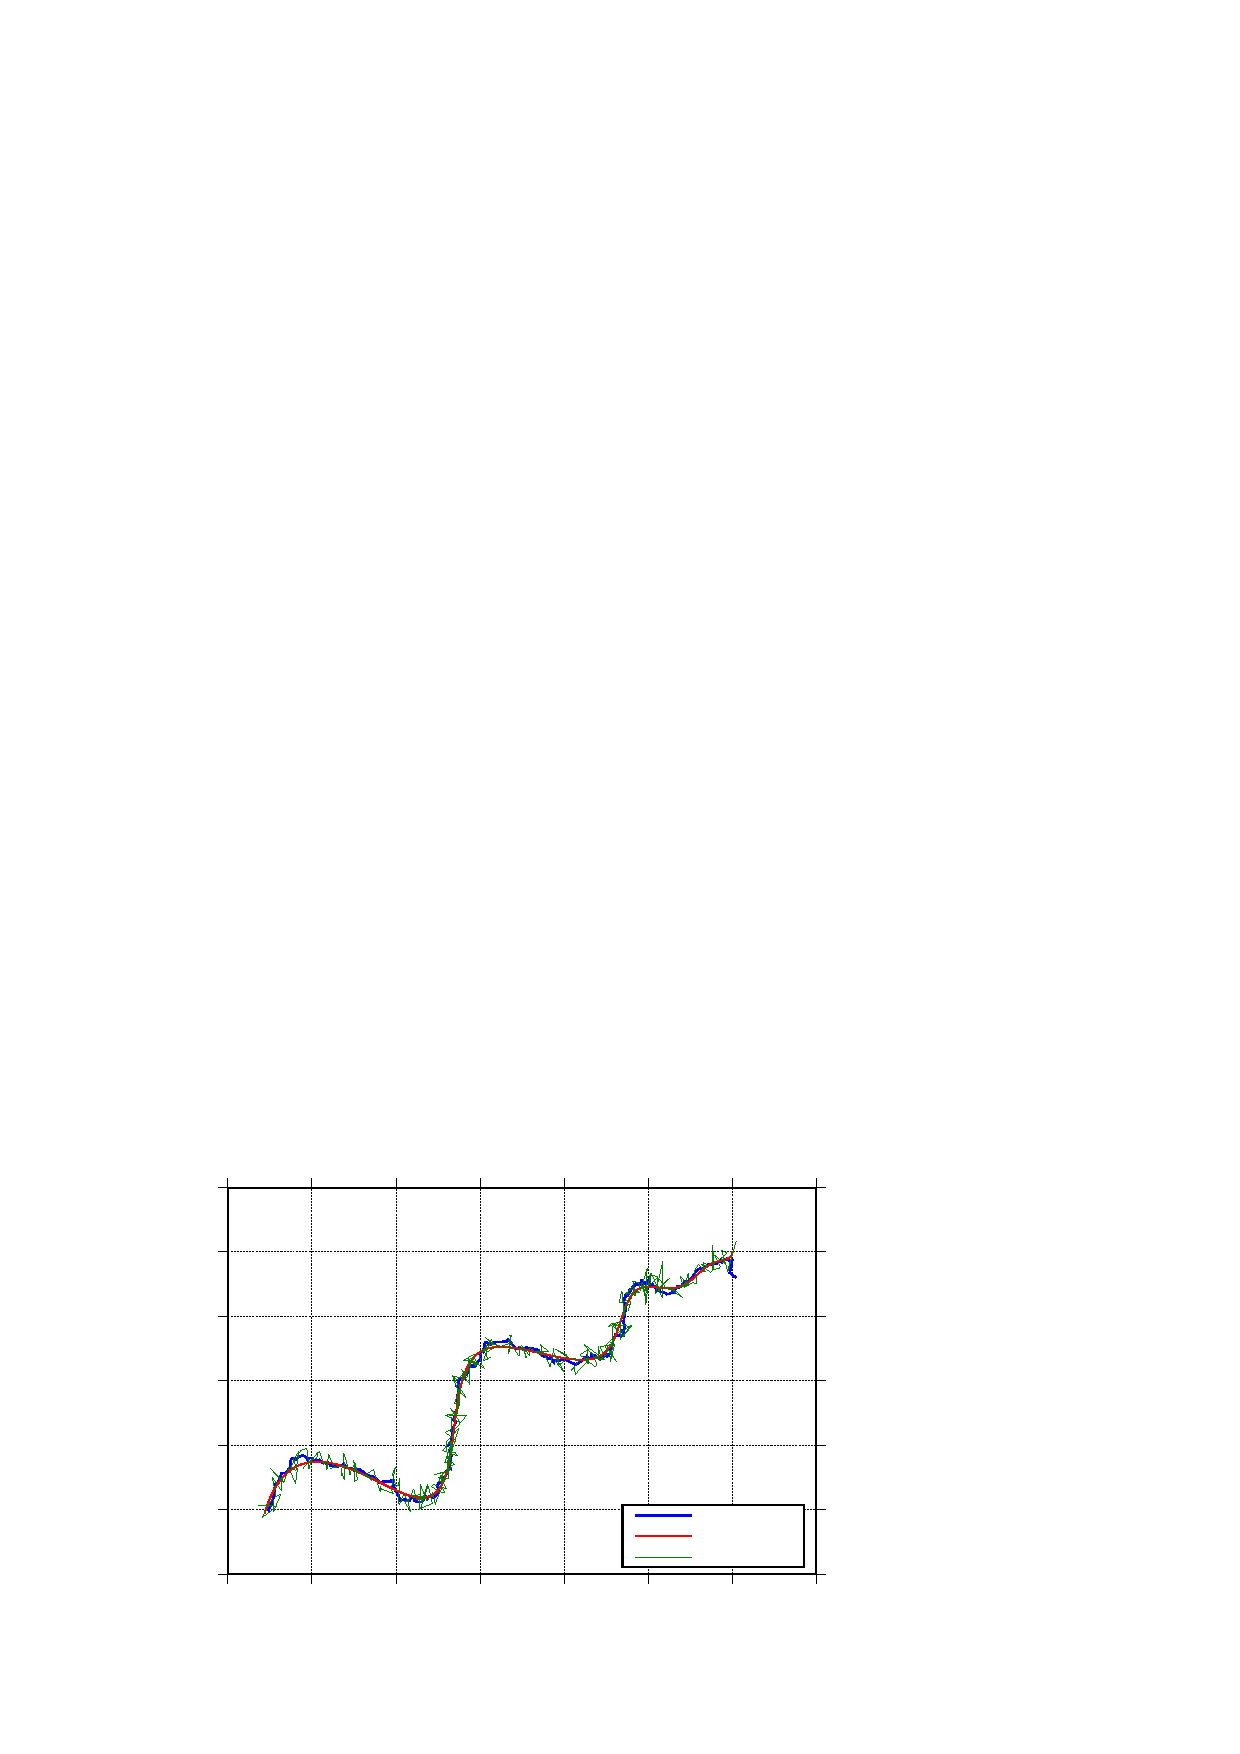
\includegraphics[width=1.0\textwidth,keepaspectratio]{Figuras/graf_ej2a.pdf}
			\caption{Caso: Medición De Posición}
			\label{fig:ej2a}
		\end{figure}
		
		En la figura \ref{fig:ej2a_innov} vemos la correlación de las innovaciones, puede verse de que se aproximan a un proceso blanco.
		
		\begin{figure}[H]
			\centering
			\includegraphics[width=1.0\textwidth,keepaspectratio]{Figuras/covinn_ej2a.pdf}
			\caption{Caso: Medición De Posición - Innovaciones}
			\label{fig:ej2a_innov}
		\end{figure}
		
		\subsubsection{Medición De Velocidad}
		
		En la figura \ref{fig:ej2b} observamos los resultados de la estimación basada en mediciones de velocidad. Puede verse que la estimación se desvía menos del valor real que las mediciones.
		
		\begin{figure}[H]
			\centering
			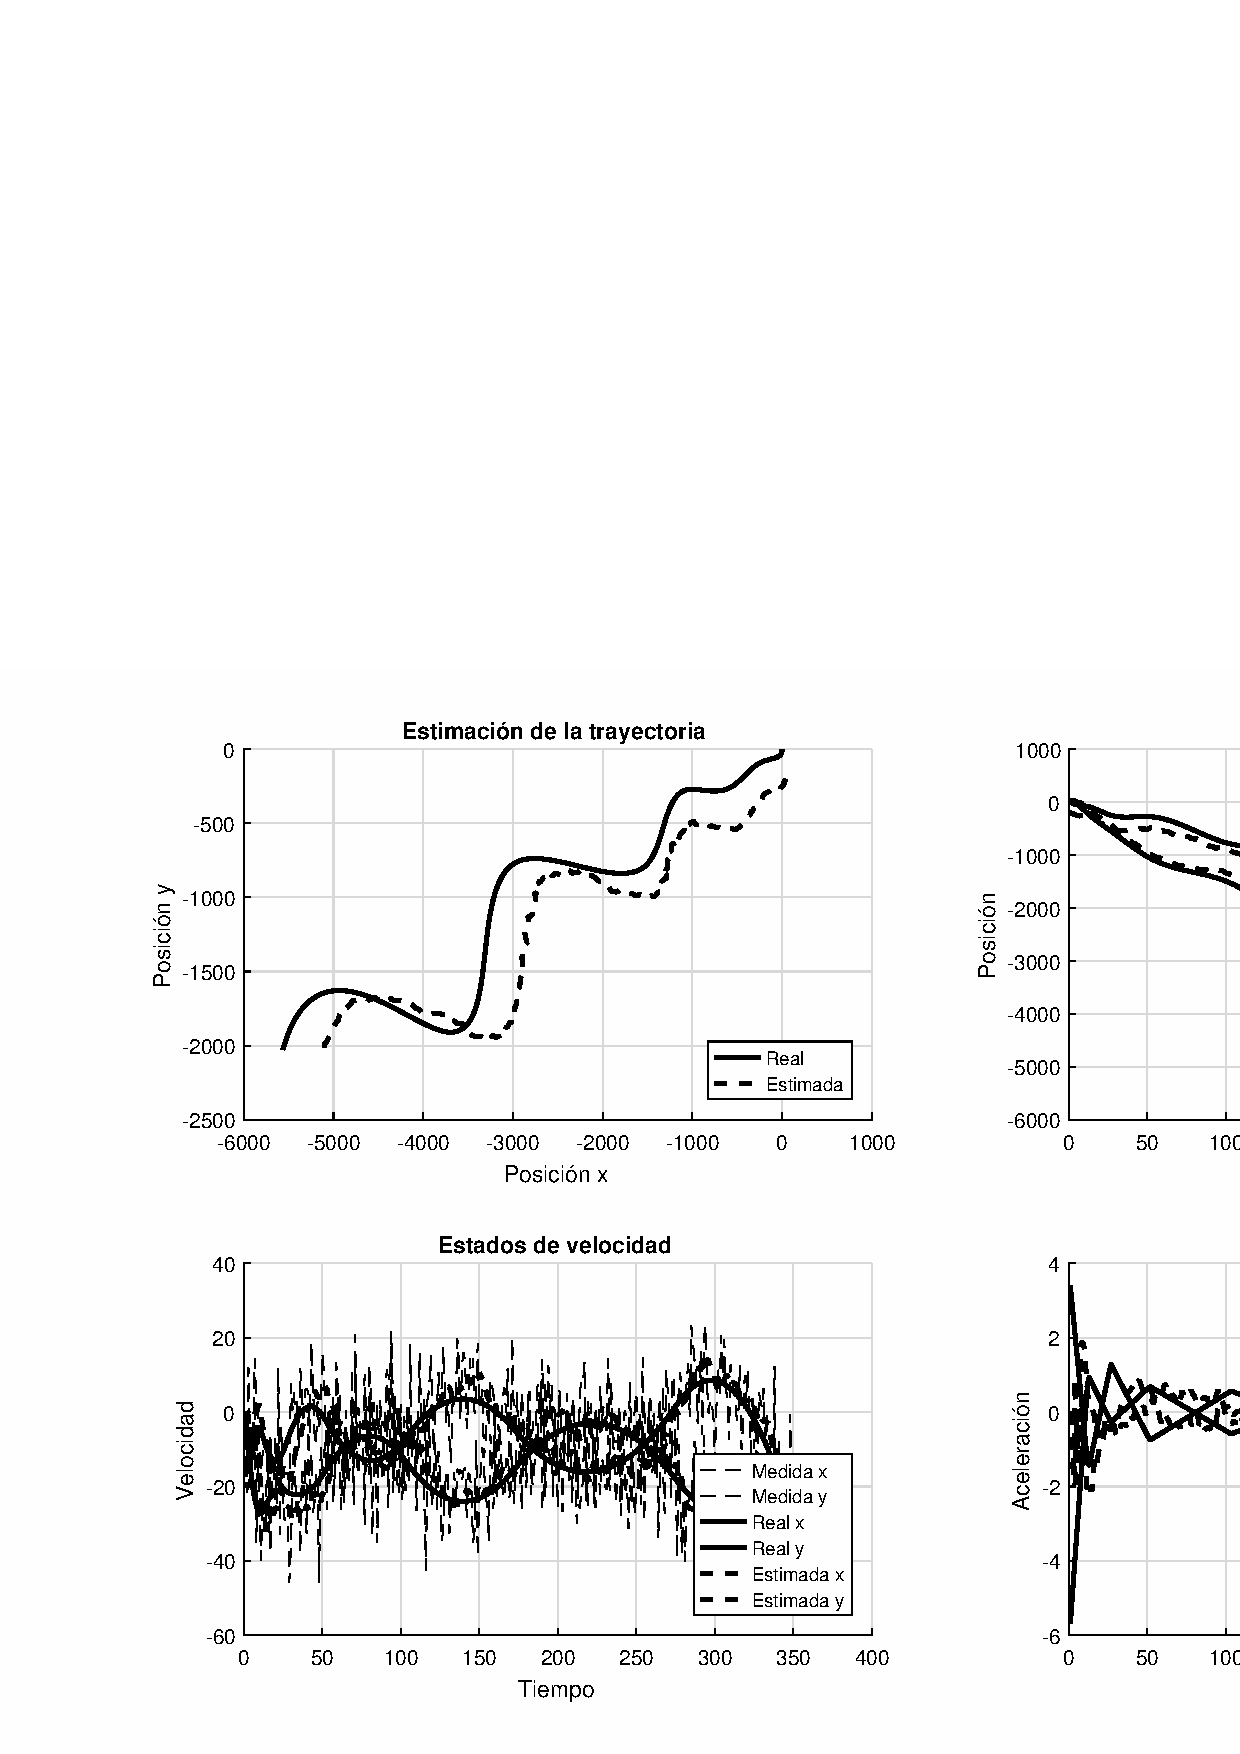
\includegraphics[width=1.0\textwidth,keepaspectratio]{Figuras/graf_ej2b.pdf}
			\caption{Caso: Medición De Velocidad}
			\label{fig:ej2b}
		\end{figure}
		
		En la figura \ref{fig:ej2b_innov} vemos la correlación de las innovaciones, puede verse de que se aproximan a un proceso blanco.
		
		\begin{figure}[H]
			\centering
			\includegraphics[width=1.0\textwidth,keepaspectratio]{Figuras/covinn_ej2b.pdf}
			\caption{Caso: Medición De Velocidad - Innovaciones}
			\label{fig:ej2b_innov}
		\end{figure}
			
		\subsubsection{Medición De Aceleración}
		
		En la figura \ref{fig:ej2c} observamos los resultados de la estimación basada en mediciones de aceleración. Puede verse que la estimación se desvía menos del valor real que las mediciones.
		
		\begin{figure}[H]
			\centering
			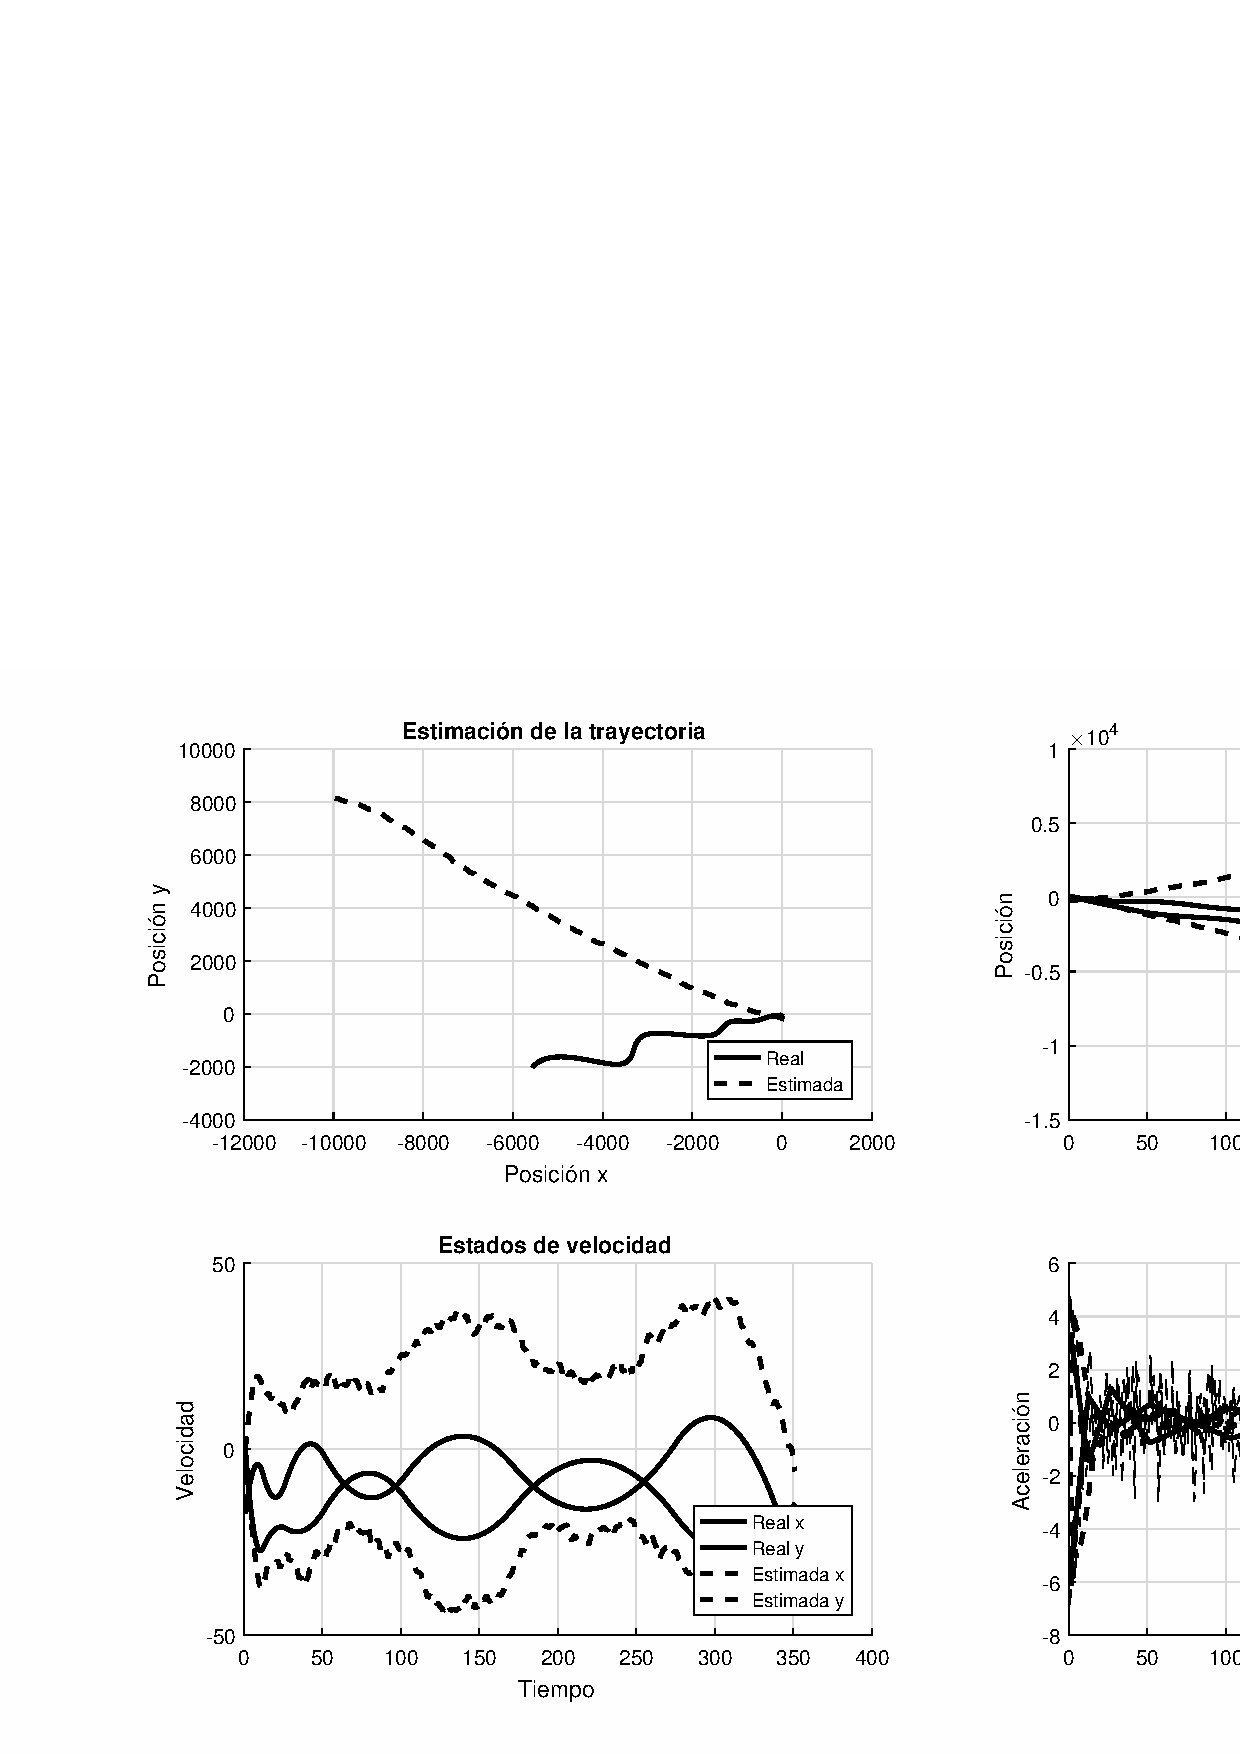
\includegraphics[width=1.0\textwidth,keepaspectratio]{Figuras/graf_ej2c.pdf}
			\caption{Caso: Medición De Aceleración}
			\label{fig:ej2c}
		\end{figure}
		
		En la figura \ref{fig:ej2c_innov} vemos la correlación de las innovaciones, puede verse de que se aproximan a un proceso blanco.
		
		\begin{figure}[H]
			\centering
			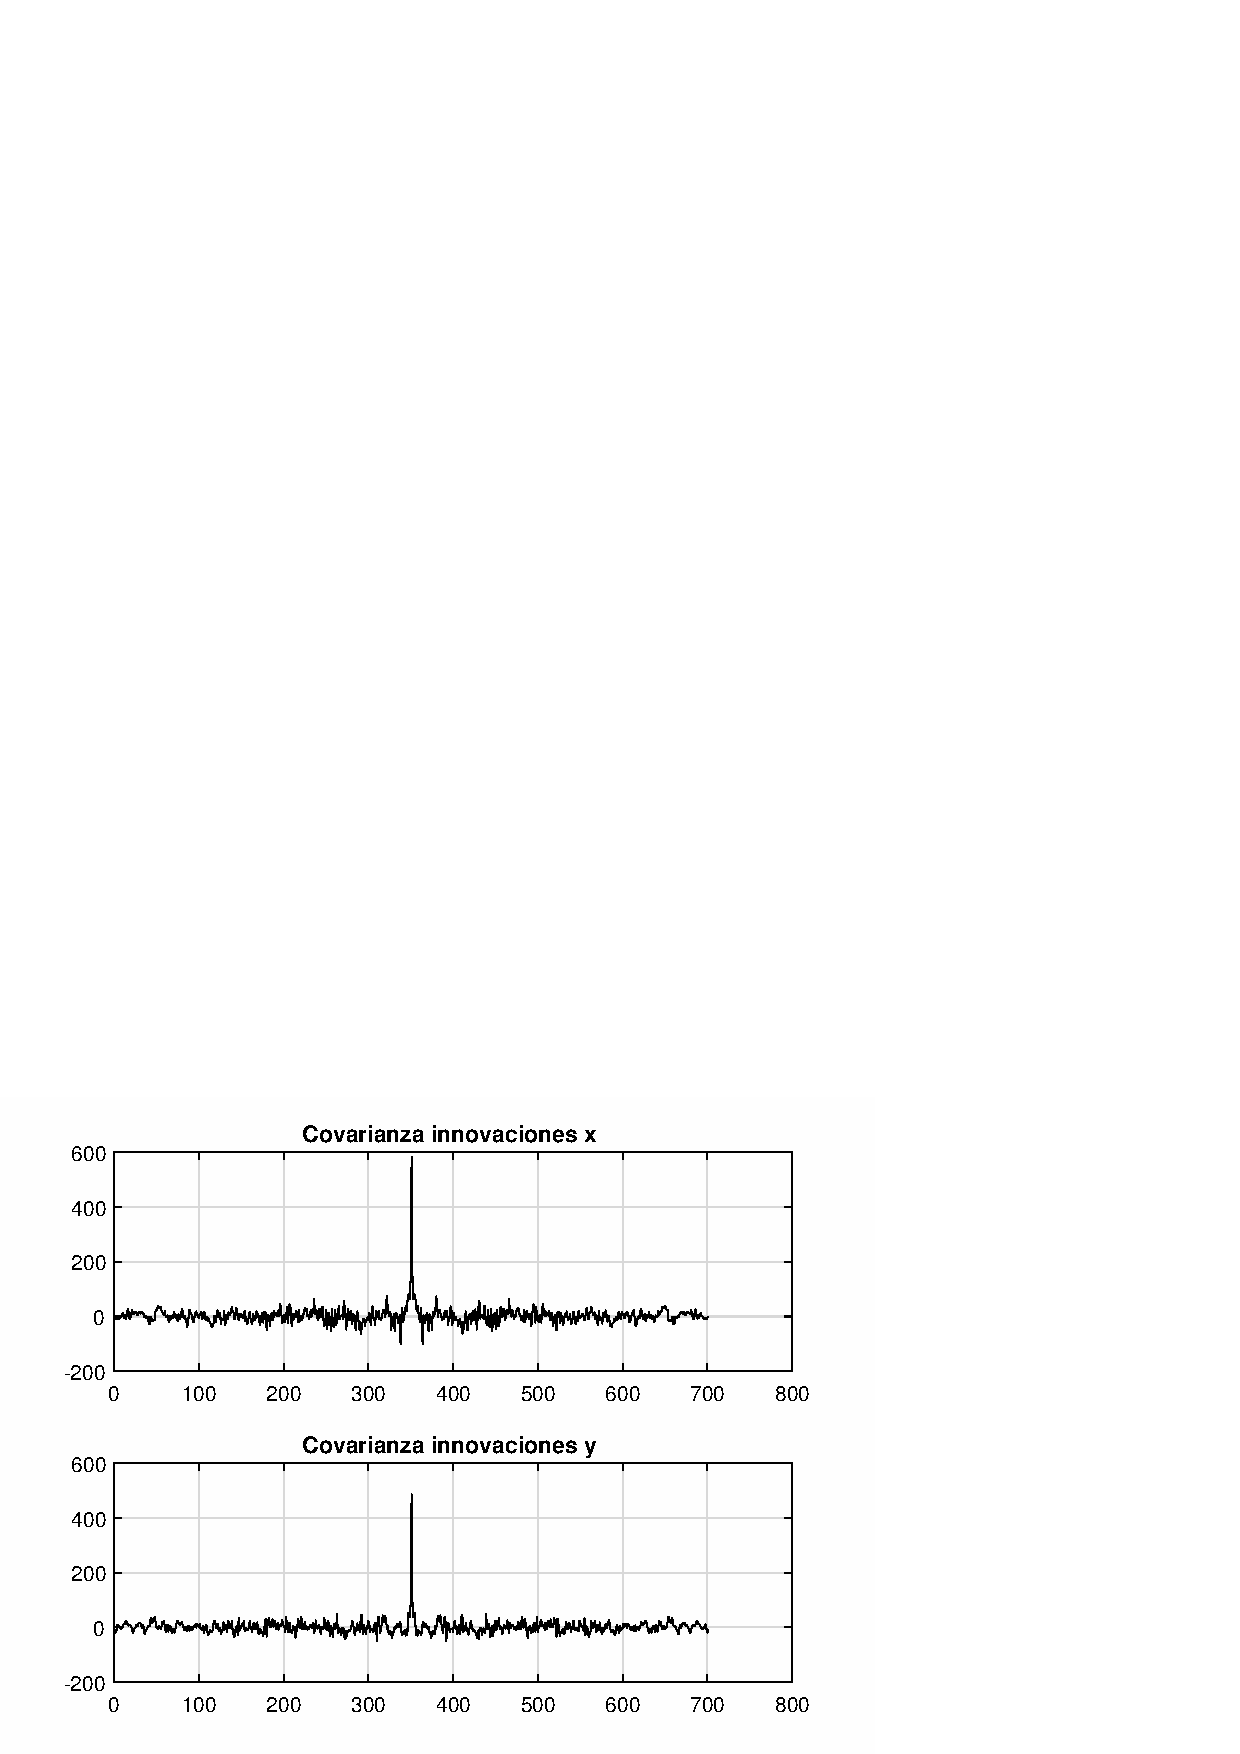
\includegraphics[width=1.0\textwidth,keepaspectratio]{Figuras/covinn_ej2c.pdf}
			\caption{Caso: Medición De Aceleración - Innovaciones}
			\label{fig:ej2c_innov}
		\end{figure}

%*% C = [eye(dim)*bool_p eye(dim)*bool_v eye(dim)*bool_a];	% Obsoleto
%*%C = [eye(dim)*bool_p eye(dim)*bool_v eye(dim)*bool_a];
%*%
%*%yk = C * ([Pos(:,1:dim) Vel(:,1:dim) Acel(:,1:dim)])' + randn(dim,cant_mediciones)*sigma_etap;

%*R = eye(dim)*sigma_etap^2;
